\documentclass{report}
\usepackage[utf8]{inputenc}
\usepackage[margin = 0.5in]{geometry}
\usepackage{ulem}
\usepackage{ragged2e}
\usepackage{graphicx}
\graphicspath{ {./images/} }

\title{\Huge\textbf{The Internet of Nano-Things}\\Article Review}
\author{Manav Karthikeyan\\AIDS - B\\21011101074}
% \date{January 2023}

\begin{document}

\maketitle
\begin{center}
    \section*{\huge\uuline{Internet of Nano-Things}}    
\end{center}
\vspace{10mm}
\section*{\uline{Summary:}}
\justifying

Nanotechnology is an area of open research which promises new non-invasive solutions for many applications in the biomedical, industrial and military fields.The interconnection of nanoscale devices with existing communication networks and ultimately the Internet defines a new networking paradigm that is further referred to as the Internet of Nano - Things.\\

This article explains upon the alternative modes of communication in the nanoscale and gives an in-depth view into this new networking paradigm from a theoretical point of view. It also discusses about the challenges faced by the nano-devices in terms of information modulation and networking protocols.

\section*{\uline{Key Concepts Discussed:}}

\subsection*{Alternative Modes of Communication at Nanoscale:}

    \begin{enumerate}
    
        \begin{description}
        
            \item[Molecular Communication] is the transmission and reception of information encoded in molecules.Molecular transceivers are expected to be easily integrated in nano-devices due to their size and domain of operation. These transceivers are able to react to specific molecules, and to release others as a response to an internal command or after performing some type of processing.
            
            \item[Nano - electromagnetic communication] is the transmission and reception of electromagnetic (EM) radiation from components based on novel nanomaterials. The unique properties observed in these materials will decide on the specific bandwidth for emission of electromagnetic radiation, the time lag of the emission, or the magnitude of the emitted power for a given input energy
            
        \end{description}
        
    \end{enumerate}

\subsection*{Network Architecture}

    The interconnection of nanomachines with existing communication networks and eventually the Internet requires the development of new network architectures. The Internet of Nano-Things can be used for two different applications:
    
    \begin{enumerate}

        \begin{description}

            \item[Intrabody Networks:]Here nanomachines such as nanosensors and nanoactuators deployed inside the human body are remotely controlled from the macroscale and over the Internet by an external user such as a healthcare provider.Amongst others, existing biological nanosensors and nanoactuators provide an interface between the biological domain and the electronic nano- devices
            
            \item[Interconnected office:]This application allows every single element normally found in an office and even its internal components are provided of a nanotransceiver which allows them to be permanently connected to the Internet. As a result, a user can keep track of the location and status of all its belongings in an effortless fashion. The possibility to harvest vibrational, mechanical or even EM energy from the environment,motivate the use of new nanomaterials in the development of these devices.
            
        \end{description}
         
    \end{enumerate}

    \begin{figure}[h]
        \centering
        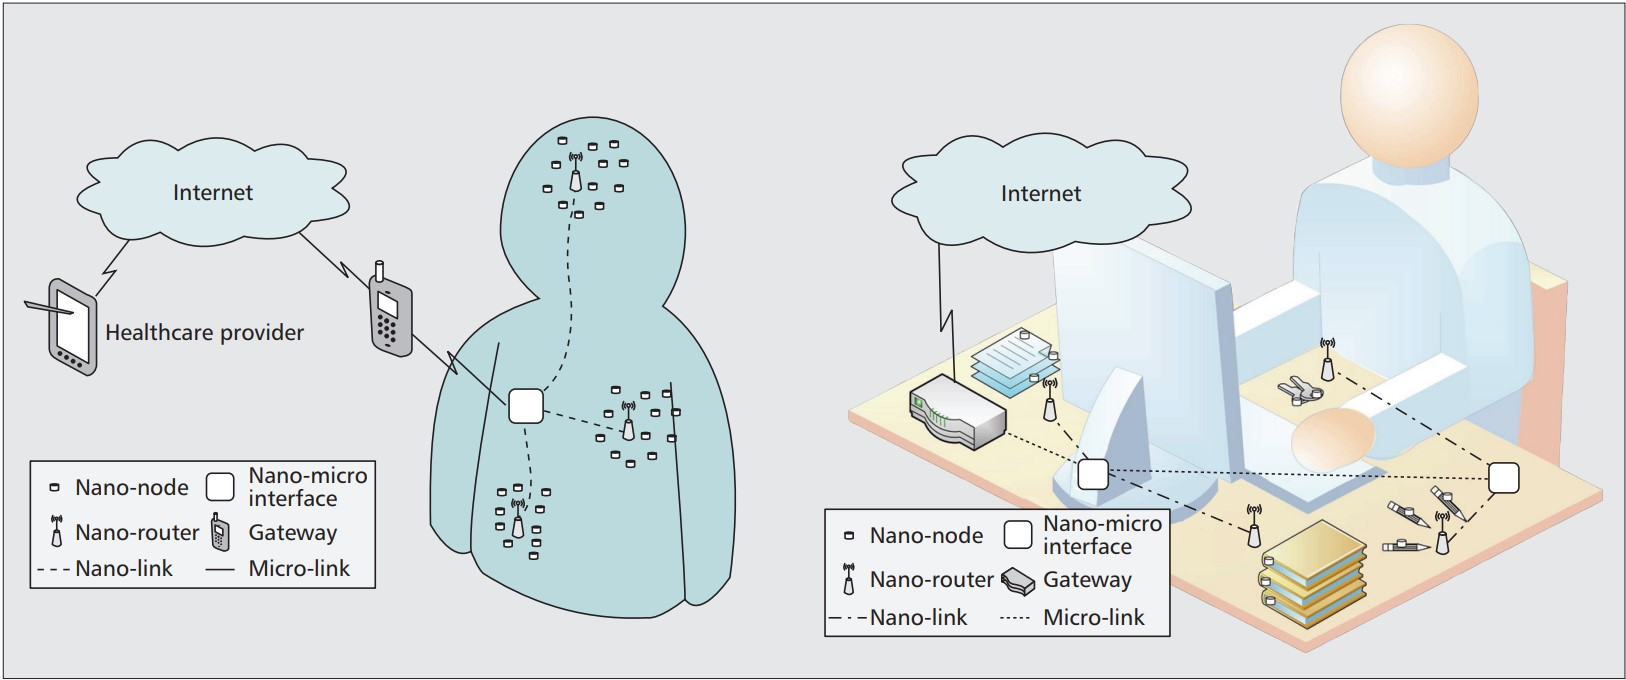
\includegraphics[width=12cm]{img.jpg}
        \caption{Network Architecture for: \textit{a) }Intrabody Networks for healthcare applications; \textit{b) }The Interconnected Office}
        \label{fig:my_label}
    \end{figure}

\subsection*{Components of Network Architecture:}

    \begin{enumerate}
        \item \textsc{Nano-nodes} are the smallest and simplest nanomachines. They are able to perform simple computation, have limited memory, and can only transmit over very short distances, mainly because of their reduced energy and limited communication capabilities.
        
        \item \textsc{Nano-routers} have comparatively larger computational resources than nano-nodes and are suitable for aggregating information coming from limited nanomachines. In addition, nano-routers can also control the behavior of nano-nodes by exchanging very simple control commands (on/off, sleep, read value, etc.)
        
        \item \textsc{Nano-micro interface devices} are able to aggregate the information coming from nanorouters, to convey it to the microscale, and vice versa. We think of nano-micro interfaces as hybrid devices able both to communicate in the nanoscale using the aforementioned nanocommunication techniques and to use classical communication paradigms in conventional communication networks.
    \end{enumerate}

\subsection*{Frequency Band of Operations:}
    The frequency band of operation for nano-transceivers and nano-antennas determines communication opportunities and challenges at the nanoscale. Graphene-based nano-antennas have been proposed, with resonant frequencies that can be up to two orders of magnitude below non-carbon materials. These antennas are efficient at radiating in the Terahertz range, matching initial predi1ctions for graphene-based RF transistors. However, the energy efficiency of mechanically resonating CNTs to generate EM waves in a nano-device is low, and future electromagnetic nanonetworks are expected to operate in the Terahertz band. A research challenge is to develop new channel models for the Terahertz band.

\subsection*{Channel Modeling:}

    Nanonetworks within the Internet of Nano-Things paradigm require an understanding of the Terahertz channel for very short range distances, below 1 meter. The properties of the Terahertz band are as follows:

    \begin{enumerate}
        \begin{description}
            \item[Path Loss - ]The total path-loss for a traveling wave in the Terahertz band is contributed by the spreading loss and the molecular absorption loss.
            \item[Noise - ]The ambient noise in the Terahertz channel is mainly contributed by the molecular noise.
            \item[Bandwidth and Chanel Capacity - ]Molecular absorption determines the usable bandwidth of the Terahertz channel. Therefore, the available bandwidth depends on the molecular composition of the channel and the transmission distance. The predicted channel capacity of electromagnetic nanonetworks in the Terahertz band is promisingly very large, in the order of a few terabits per second.
        \end{description}
    \end{enumerate}

    However, the very limited capabilities of individual nanomachines question the reproducibility of these results in a real implementation. In other words, the information capacity is mostly limited by the capabilities of nanomachines rather than by the channel itself.

\subsection*{Information Modulation:}

    A new communication paradigm for nanomachines is proposed based on the exchange of very short pulses, just a few femtoseconds long, to take advantage of the huge bandwidth provided by the Terahertz channel. The key ideas of this new communication paradigm are as follows:
    \begin{enumerate}
        \item Transmission of short pulses
        \item Pulse-based communications
        \item Modulation of the amplitude, temporal position, duration, time between, or rate of the transmitted pulses
        \item Transmission of multiple pulses in a burst to relax detection requirements
        \item Optimization of parameters such as energy per pulse, number of pulses in a burst, and time between consecutive pulses in a cross-layer fashion
        \item A packet composed of a fixed number of symbols spaced in time, with a time between symbols much larger than the symbol duration to address the limited power options for nanomachines.
    \end{enumerate}

\subsection*{Protocols for Nanonetworks:}

    The authors propose a new communication paradigm for nanonetworks based on the exchange of very short pulses, just a few femtoseconds long, using a time spread on-off keying modulation. They suggest that different channel access mechanisms for nanonetworks need to be defined depending on how the information is encoded. They propose the use of asynchronous MAC protocols and interleaving different pulse streams to reduce chances of collisions. They also suggest a more relaxed approach to assigning unique IDs to nano-nodes in order to simplify synchronization and coordination. They also note that the number of neighboring nano-nodes that can potentially interfere with a specific user is not as large due to their limited transmission power and high frequencies. These concepts are proposed as a starting point for the development of MAC protocols for nanonetworks.

\subsection*{My Views (Agreements and Pitfalls):}
    To start off, even though this article~\cite{5675779} was published 10 years back, right around when IoT was starting to gain momentum, the authors were able to correctly predict the direction this specific domain was headed.\\\\
    However recent technological advancements have helped improve the prospects of incorporating nanotechnology into our daily lives and also integrating them onto the Internet. For example, graphene-based nanoantennas, have allowed for the creation of small, low-power, and highly sensitive nanodevices that can be integrated into various systems. Additionally, the use of pulse-based communication techniques, such as Impulse Radio Ultra-Wide-Band (IR-UWB), has further optimized the communication capabilities of these devices.\\

    The authors had also mentioned that vibrational, mechanical and even electromagnetic energy could possibly be harnessed to power these nano-devices. I could not agree more with this point, in fact vibrational/thermal energy seems to be an excellent energy source for these devices due to the abundance of thermal energy lost/released in biological phenomenon and in electronic objects. This is not only a renewable source of energy but it also helps in minimizing the energy lost as heat.\\

    However, on the other hand, there are still significant challenges that need to be addressed before the widespread adoption of nanotechnology can occur. One of the major challenges is the development of robust and efficient communication protocols for these devices, as the limited hardware capabilities of nano-devices make it difficult to implement traditional communication methods. Additionally, the development of efficient and reliable addressing and identification systems for these devices is also a major challenge. Furthermore the abscense of encryption capabilities within these nano-devices due to lack of computational power is a major security concern.\\

    In conclusion, while the Internet of Nano Things holds great potential for revolutionizing various industries, significant challenges need to be addressed before the widespread adoption of these devices can occur. However, recent advancements in nanotechnology and communication techniques have provided a foundation for the development of efficient and reliable systems, and ongoing research in this field is expected to lead to further breakthroughs in the near future.

\bibliographystyle{plain}
\bibliography{citation.bib}
\end{document}
